

\begin{frame}
  \frametitle{Ranking with ERK Signalling}
  \begin{itemize}
  \item Target Ranking for Elk-1.
  \item Elk-1 is phosphorylated by ERK from the EGF signalling pathway.
  \item Predict concentration of Elk-1 from known targets.
  \item Rank other targets of Elk-1.
  \end{itemize}

\end{frame}


\begin{frame}
  \frametitle{Elk-1 (MLP covariance)}

  \begin{flushright}
    \textbf{Jennifer Withers}
    \par\end{flushright}

  % 
  \begin{figure}
    \centering{}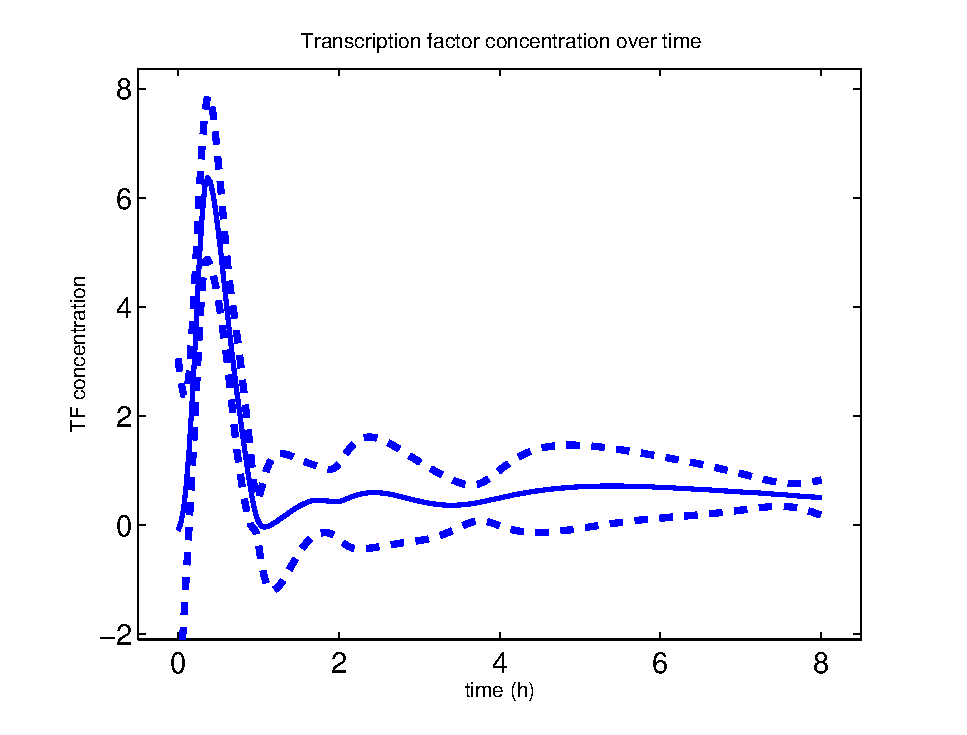
\includegraphics[width=0.3\textwidth]{../../../gpsim/tex/diagrams/MLP_TFConcentration}\hfill{}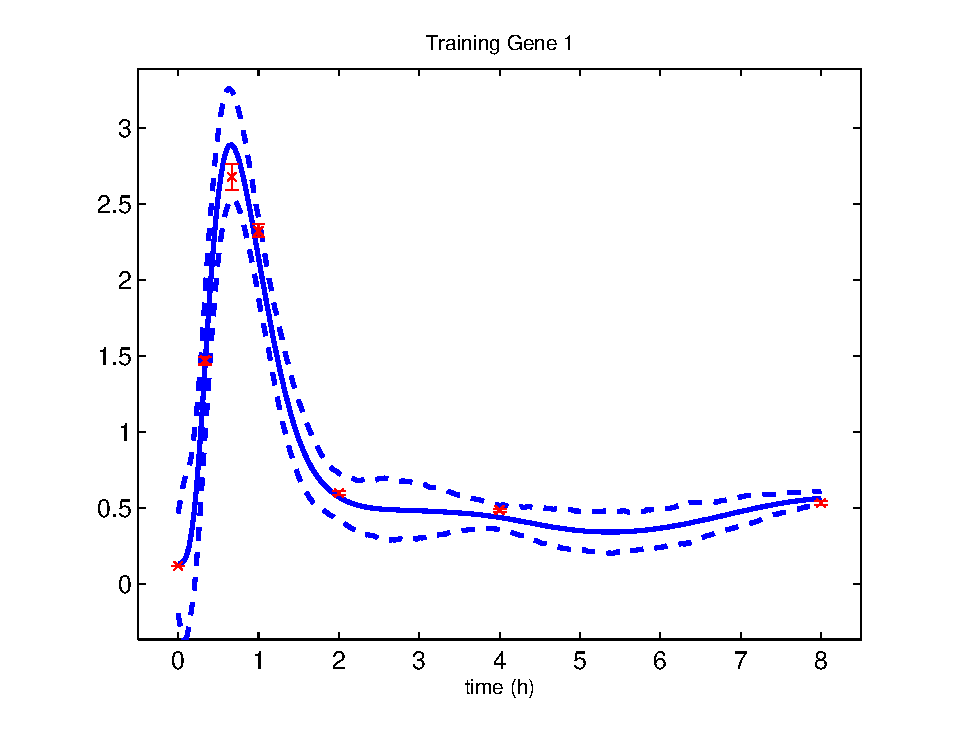
\includegraphics[width=0.3\textwidth]{../../../gpsim/tex/diagrams/MLP_TrainingGene1}\hfill{}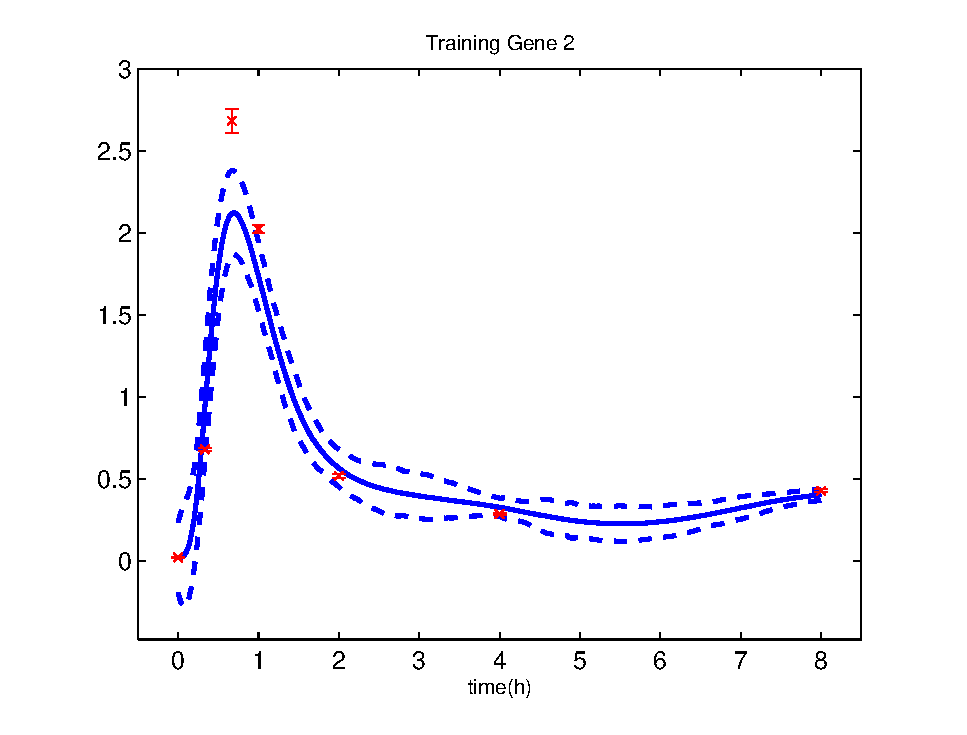
\includegraphics[width=0.3\textwidth]{../../../gpsim/tex/diagrams/MLP_TrainingGene2}\\
    \includegraphics[width=0.3\textwidth]{../../../gpsim/tex/diagrams/MLP_TrainingGene3}\hfill{}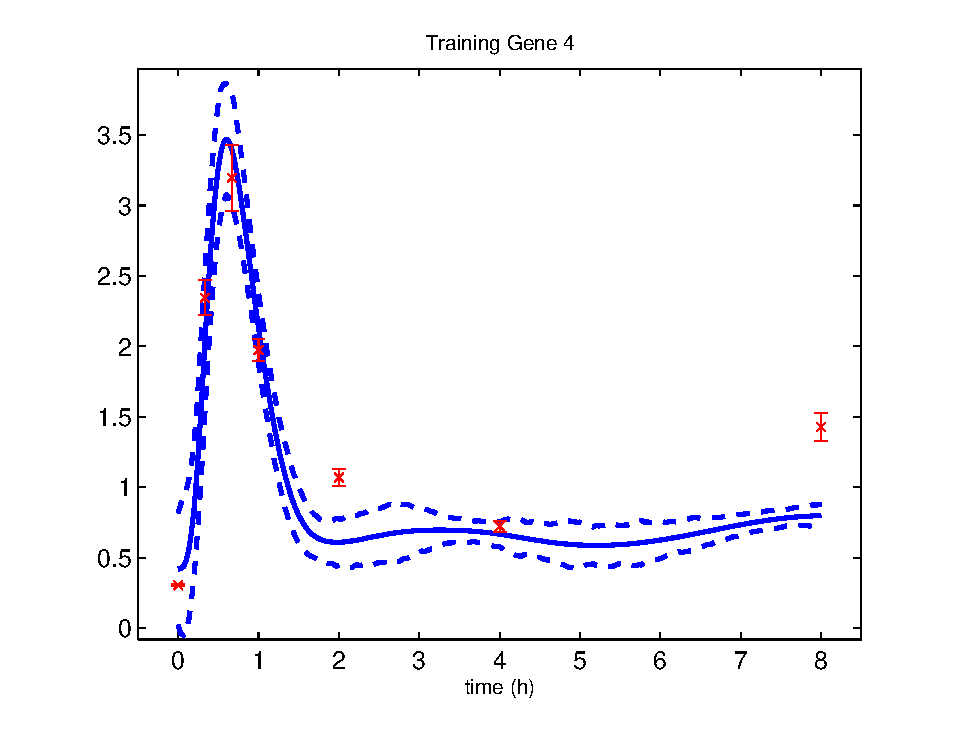
\includegraphics[width=0.3\textwidth]{../../../gpsim/tex/diagrams/MLP_TrainingGene4}\hfill{}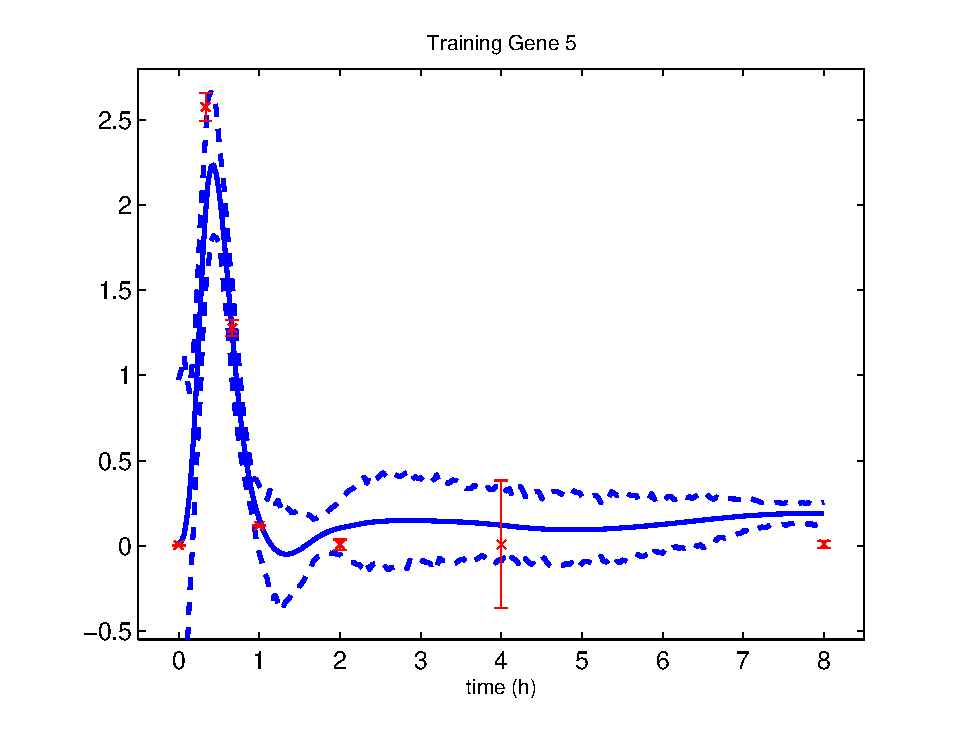
\includegraphics[width=0.3\textwidth]{../../../gpsim/tex/diagrams/MLP_TrainingGene5}
  \end{figure}

\end{frame}

\begin{frame}
  \frametitle{Elk-1 target selection}

  Fitted model used to rank potential targets of Elk-1
  \begin{columns}[c]%{}


    \column{2.5 in}

    % 
    \begin{figure}
      \centering{} 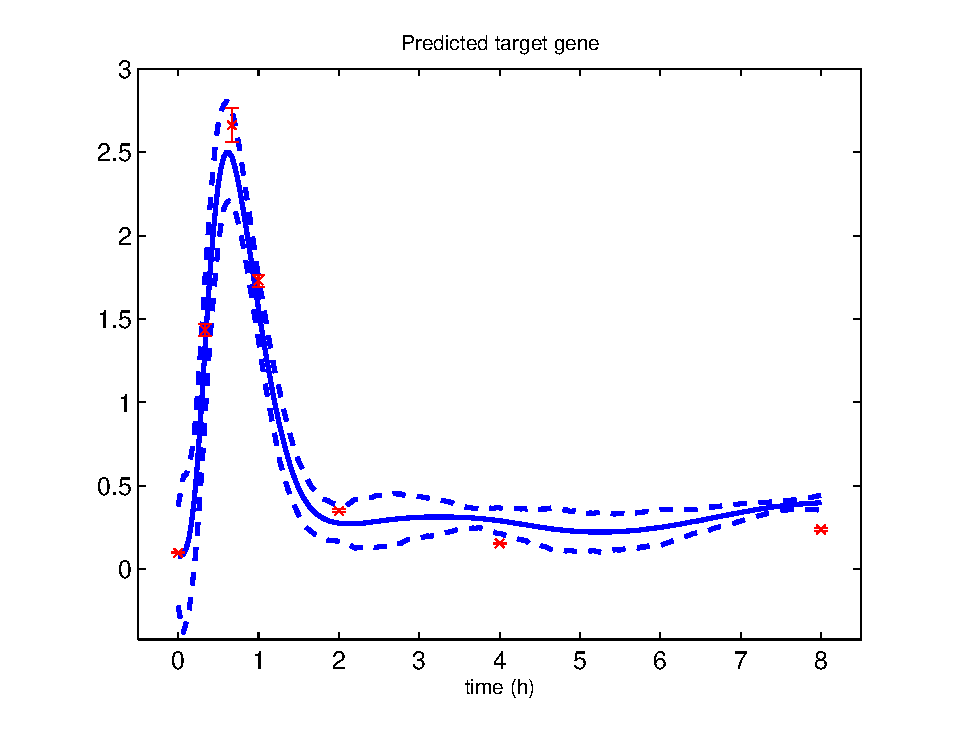
\includegraphics[width=7cm]{../../../gpsim/tex/diagrams/MLP_GoodFit} 
    \end{figure}


    \centering


    \column{2.5 in}

    % 
    \begin{figure}
      \centering{} 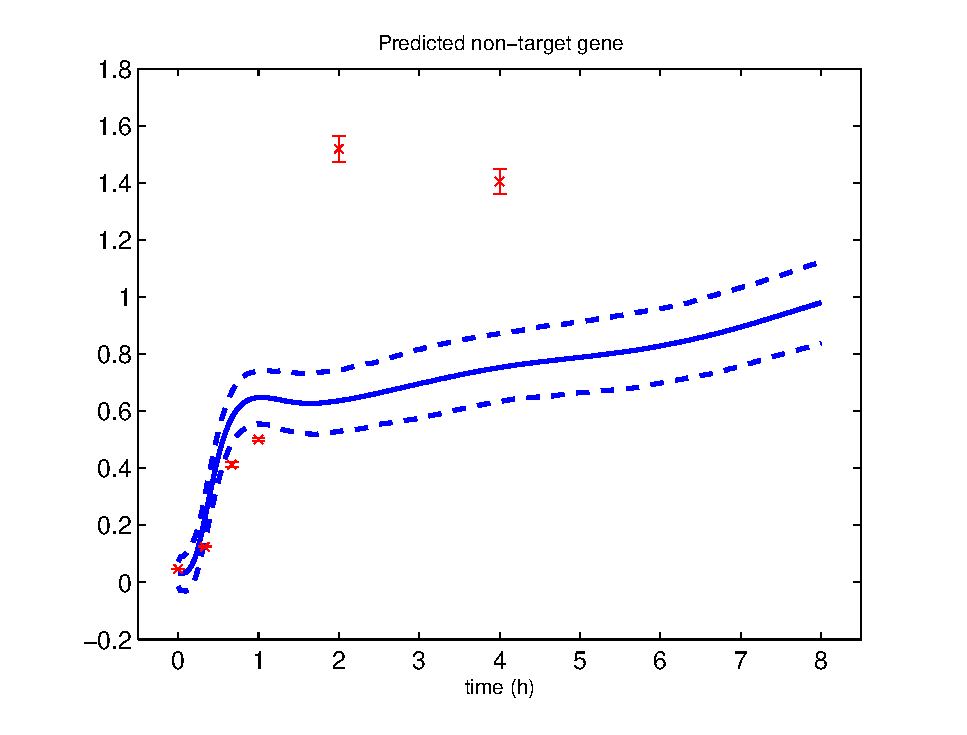
\includegraphics[width=7cm]{../../../gpsim/tex/diagrams/MLP_BadFit} 
    \end{figure}


  \end{columns}%{}

\end{frame}


